\chapter{Manual del usuario}

\section{Visión general}

\subsection{Introducción}

En el siguiente documento se recoge una descripción del funcionamiento del simulador de escenarios con usuarios móviles para la evaluación de algoritmos de recomendaciones.

\subsection{¿Que es el simulador de escenarios con usuarios móviles?}

El simulador de escenarios con usuarios móviles es una herramienta que trata de simular distintos tipos de algoritmos de recomendaciones en el entorno de una ciudad real con el fin de evaluar su correcto funcionamiento.

Se trata de un sistema multiusuario donde distintos tipos de usuarios se conectan y se mueven en una ciudad real (el entorno es configurado de antelación). El recomendador tiene en cuenta distintos tipos de parámetros: desde sus posiciones geográficas hasta sus perfiles y preferencias.

\subsection{Tipos de tecnologías utilizadas}

Esta herramienta consta de dos partes: la primera es el simulador y la segunda es el recomendador.

El Simulador esta desarrollado con nodejs, sockets-io, angularjs, bootstrap y como base de datos utiliza mongodb. El recomendador está desarrollado con java. La integración entre el navegador (cliente), simulador y recomendador está realizada mediante un sistema de evetos bidireccionales (sockets-io). De esta forma conseguimos comunicar todas la partes del sistema en tiempo real.

\subsection{Instalación}

\subsubsection{Paso 1: Instalar mongoDB}

Lo primero que tenemos que hacer es instalar mongodb. Los pasos para la instalación de mongodb depeden del tipo de sistema operativo que disponemos. Por esto no vamos a entrar en detalle de como se instala y vamos a seguir el tutorial disponible en la web oficial:

\begin{itemize}
	\item Linux: https://docs.mongodb.org/manual/administration/install-on-linux/
	\item Windows: https://docs.mongodb.org/manual/tutorial/install-mongodb-on-windows/
	\item Mac OS: https://docs.mongodb.org/manual/tutorial/install-mongodb-on-os-x/
\end{itemize}

\subsubsection{Paso 2: Instalar Node.js y NPM}

Vamos en la web oficial de nodejs (https://nodejs.org) y descargamos e instalamos la version v0.12.4. En el caso de Windows la instalación es igual que la de cualquier otro programa. Para la instalación en otros SO visitar https://nodejs.org/en/download/.

A continuación tenemos que instalar el gestor de paquetes NPM v2.10.1. En el caso de Windows vamos en la web oficial (https://nodejs.org/en/download/) y nos descargamos e instalamos el ejecutable. En el caso de Linux ejecutamos el siguiente comando en la consola:
\begin{lstlisting}[language=xml, frame=single]
sudo apt-get install npm
\end{lstlisting}

\subsubsection{Paso 3: Instalar git}

Git es un sistema distribuido de control de versiones. Para la instalación de este nos descargamos el ejecutable de https://git-scm.com/downloads y seguimos los pasos que nos indica este.

\subsubsection{Paso 4: Clonar el proyecto de github e instalarlo}

A continuacion tenemos que clonar el proyecto del Simulador de github. Para esto abrimos una consola y nos situamos en el directorio donde queremos clonar el proyecto. A continuacion ejecutamos el siguiente comando:
\begin{lstlisting}[language=xml, frame=single]
git clone https://github.com/slavcho87/Simulator
\end{lstlisting}
Vemos que se ha creado un directorio llamado Simulator. Lo primero que tenemos que hacer es bajarnos todas las dependencias del proyecto. Por esto ejecutamos el siguiente comando:
\begin{lstlisting}[language=xml, frame=single]
npm install
\end{lstlisting}
Una vez que nos hemos clonado el proyecto y descargado las dependencias de este podemos arrancar el servidor mediante el siguiente comando:
\begin{lstlisting}[language=xml, frame=single]
npm start
\end{lstlisting}

\paragraph{Paso 4.1: Configuraciones básicas del simulador}

En el fichero baseConfig.json disponemos de las siguientes basicas para el simulador como el puerto donde se ejecuta el servidor y la localizacion de la base de datos. Si editamos el fichero baseConfig.json veremos que tiene el siguiente contenido:
\begin{lstlisting}[language=xml, frame=single]
{ 
"port": 81, 
"locationDB": "localhost", 
"nameDB": "simulator" 
}
\end{lstlisting}

Las variables del fichero baseConfig.json tienen el siguiente significado:

\begin{itemize}
	\item port: es el puerto donde se va a ejecutar el servidor
	\item locationDB: es la localizacion donde se va a ejecutar mongodb.
	\item nameDB: es el nombre del esquema de la base de datos donde nos conectamos.
\end{itemize}

Dichas configuraciones son importantes ya que de esta forma tenemos la opción de llevarnos la base de datos en un servidor diferente para darle más potencia.

\paragraph{Paso 4.2: Posibles problemas durante la ejecución del simulador}

Se puede dar el caso que al intentar arrancar el simulador nos de el siguiente error:

\begin{lstlisting}[language=xml, frame=single]
Error: listen EACCES 0.0.0.0:81
at Object.exports._errnoException (util.js:870:11)
at exports._exceptionWithHostPort (util.js:893:20)
at Server._listen2 (net.js:1218:19)
at listen (net.js:1267:10)
at Server.listen (net.js:1363:5)
\end{lstlisting}

El error EACCES ocurre cuando no tenemos suficientes privilegios sobre el puerto donde estamos lanzando el servidor Node.js. La solución depende del Sistema Operativo que estamos usando. En el caso de Windows tenemos que cambiar el puerto donde lanzamos el servidor siempre y cuando estemos usando un usuario que tenga suficientes privilegios. En el caso de Linux tenemos que lanzar el servidor con el comando sudo delante de la siguiente manera:

\begin{lstlisting}[language=xml, frame=single]
slavcho@ubuntu:~/Simulator/scripts$ sudo ./ejecutarSimulador.sh
\end{lstlisting}

\subsubsection{Paso 5: Instalación del recomendador}

\paragraph{Paso 5.1: Instalar Apache maven}

Antes de todo tenemos que instalar Apache maven que es un gestor de paquetes. Por lo tanto vamos en la web oficial (https://maven.apache.org/) y descargamos y descomprimimos el ficheros compromido. A continuación tenemos que añadir en la variable PATH la dirección de la carpeta donde hemos descomprimido maven. Para ver que maven se haya instalado correctamente ejecutamos el siguiente comando:
\begin{lstlisting}[language=xml, frame=single]
mvn -v
\end{lstlisting}
De esta forma comprobamos la version de maven que tenemos instalado. Tenemos que ver una salida como la siguiente: \newline

\begin{lstlisting}[language=xml, frame=single]
Apache Maven 3.2.5 (12a6b3acb947671f09b81f49094c53f426d8cea1; 2014-12-14T18:29:23+01:00)
Maven home: C:\maven
Java version: 1.7.0_79, vendor: Oracle Corporation
Java home: C:\Program Files (x86)\Java\jdk1.7.0_79\jre
Default locale: es_ES, platform encoding: Cp1252
OS name: "windows 8.1", version: "6.3", arch: "x86", family: "windows"
\end{lstlisting}

\paragraph{Paso 5.2: Compilar el recomendador}

Una vez que hayamos instalado maven correctamente tenemos que compilar el recomendador. Por esto ejecutamos el ficheros compilarRecommender que se encuentra en la carpeta scripts. Existen dos versiones: uno para Windows y otro para Linux.

\paragraph{Paso 5.3: Configuraciones básicas del recomendador}

Si editamos el fichero configs/baseConfig.txt podemos ver que tiene el siguiente formato:
\begin{lstlisting}[language=xml, frame=single]
<config>
<host>http://localhost</host>
<port>81</port> 
<hostMongo>localhost</hostMongo>
<portMongo>27017</portMongo> 
<nameDB>simulator</nameDB> 
</config>
\end{lstlisting}

\begin{itemize}
	\item host: es la dirección donde se ejecuta el simulador. En el ejemplo este se está ejecutando en local
	\item port: es el puerto donde se ejecuta el simulador. En el ejemplo este se ejecuta en el puerto 81
	\item hostMongo: es la dirección de la base de datos. En el ejemplo esta se está ejecutando en local
	\item portMongo: es el puerto donde se ejecuta la base de datos.
	\item nameDB: es el nombre del esquema de la base de datos
\end{itemize}

\paragraph{Paso 5.4: Ejecutar el recomendador}

Para ejecutar el recomendar tenemos que ejecutar el ficheros ejecutarRecommender que se encuentra en la carpeta scripts. Existe dos versiones de este fichero: uno para Windows y otro para Linux.

\subsection{Primeros pasos}

El primero paso al instalar el simulador es crear nuestro usuario (apartado \ref{sec:CrearUsuario}). A continuación vamos en Settings y realizamos las configuraciones realizadas en los capítulos \ref{sec:confRecomendador}, \ref{sec:confObjEstaticos} y \ref*{sec:confObjDinamicos}.

Se trata de crear nuevas configuraciones para el recomendador y crear los tipos de objetos dinámicos y estáticos que usaremos posteriormente en la creación de mapa (apartado \ref{sec:crearMapa}) y escenas (apartado \ref{sec:crearEscena}).

\section{Configuración del recomendador}\label{sec:confRecomendador}

Para configurar los parámetros del recomendador primero tenemos que estar autentificados con nuestros usuario. Una vez autentificados vamos en Settings $\rightarrow$ Recommender settings y vemos la siguiente pantalla:

\begin{figure}[H]
	\centering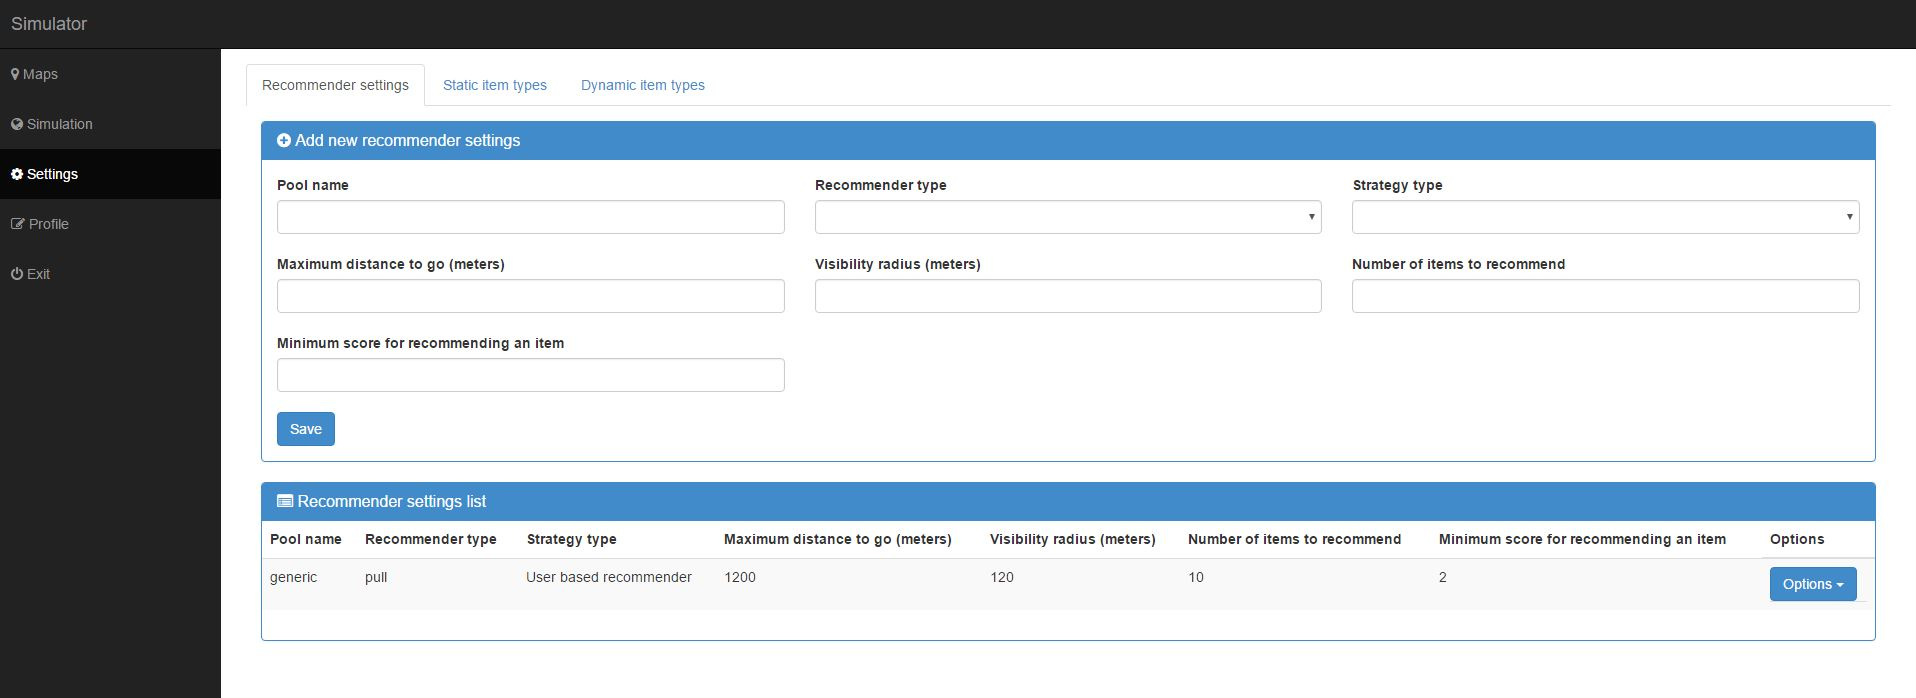
\includegraphics[scale=0.35]{imagenes/capitulo2/configuracion-recomendador.jpg}
	\caption{Configuración del recomendador}
	\label{img:ConfiguracionRecomendador}
\end{figure}


En este formulario tenemos que introducir los siguientes datos:
\begin{itemize}
	\item Pool name: es nombre que vamos a dato al conjunto de parámetros
	\item Recommender type: es el tipo de recomendador. Podemos elegir entre pull (el usuario solicita una recomendación) o push (el recomendador realiza recomendaciones sin que el usuario lo haya solicitado)
	\item Strategy type:: indicar el tipo de implementación que queremos para el recomendador
	\item Maximum distance to go (meters): es la distancia máxima (en metros) que está dispuesto a recorrer el usuario
	\item Visibility radius (meters): radio (en metros) de visibilidad del usuario. Los items que están fuera de este radio son invisibles para el usuario 
	\item Number of items to recommend: número máximo de items que va a recomendar el recomendador cada vez
	\item Minimum score for recommending an item: puntuación mínima para que un item sea recomendado
\end{itemize}

\newpage

\section{Configuración de los objetos estáticos}\label{sec:confObjEstaticos}

Para crear un nuevo tipo de objeto estático primero tenemos que estar autentificados con nuestros usuario. Una vez autentificados vamos en Settings $\rightarrow$ Static item type y vemos la siguiente pantalla:

\begin{figure}[H]
	\centering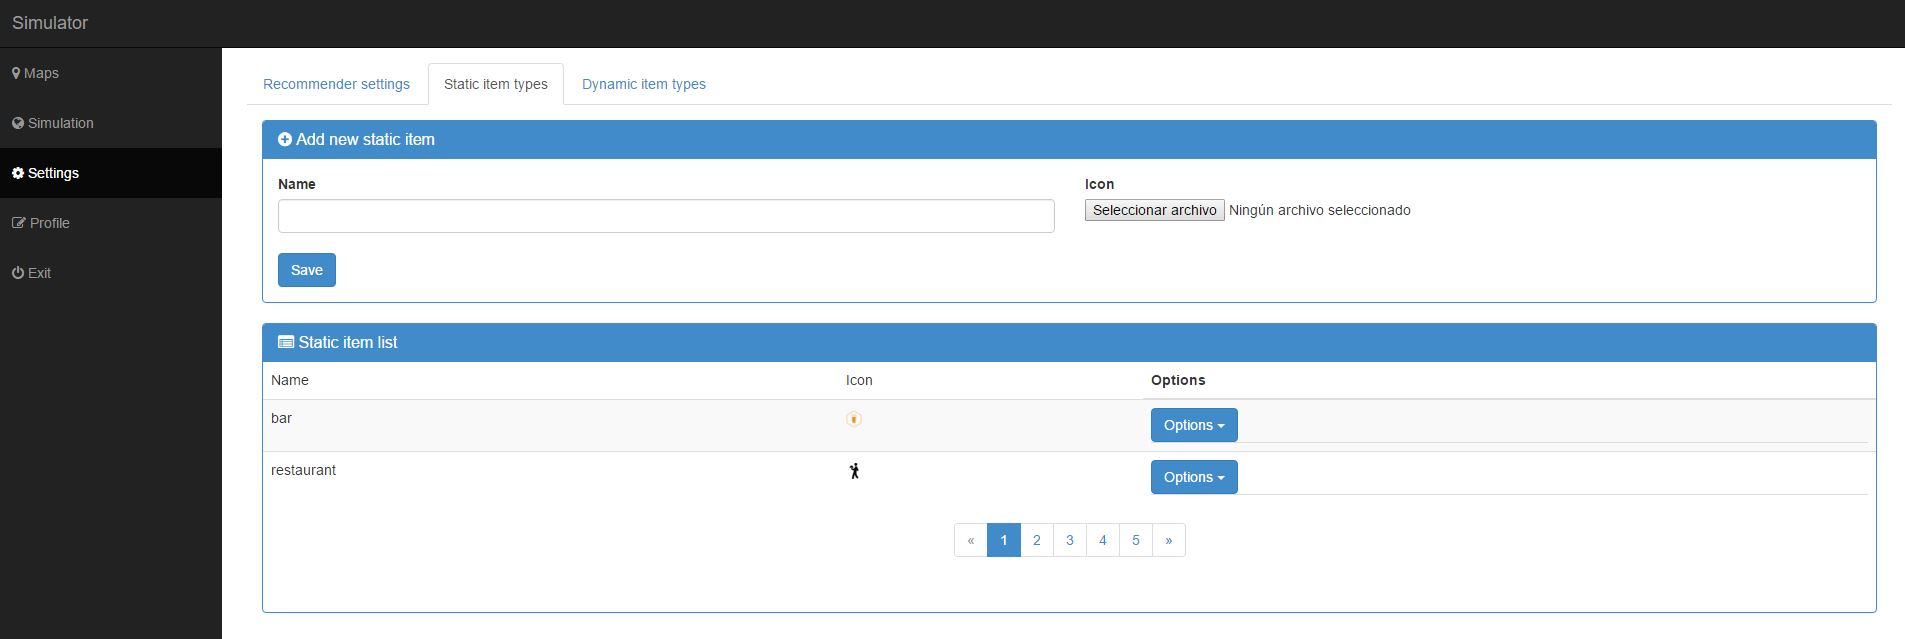
\includegraphics[scale=0.35]{imagenes/capitulo3/config-objetos-estaticos.jpg}
	\caption{Configuración de los objetos estáticos}
	\label{img:ConfiguracionObjetosEstaticos}
\end{figure}

En este formulario tenemos que introducir los siguientes datos:

\begin{itemize}
	\item Name: es el nombre del tipo del objeto estático
	\item Icon: icono del tipo del objeto estático
\end{itemize}	

Por debajo del formulario de creación nuevos tipos de objetos estáticos aparecerá la lista con todos los tipos de objetos estáticos que han sido creados. En el apartado opciones podemos gestionar cada uno de estos objeto.

\section{Configuración de los objetos dinámicos}\label{sec:confObjDinamicos}

Para crear un nuevo tipo de objeto dinámicos primero tenemos que estar autentificados con nuestros usuario. Una vez autentificados vamos en Settings $\rightarrow$ Dynamic item type y vemos la siguiente pantalla:

\begin{figure}[H]
	\centering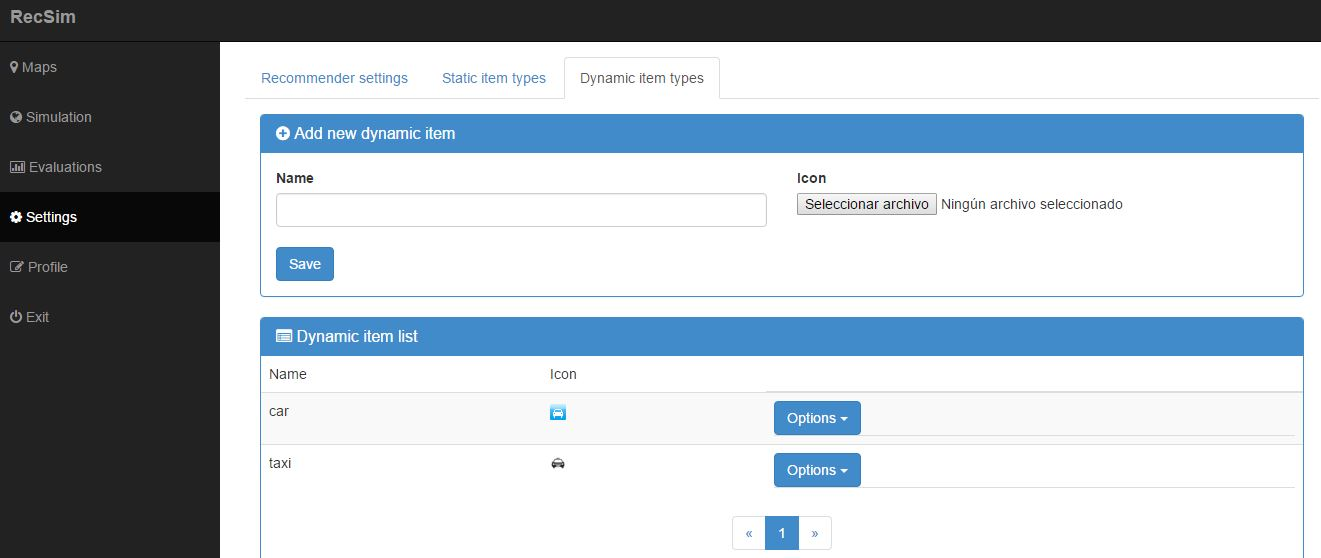
\includegraphics[scale=0.35]{imagenes/capitulo4/config-objetos-dinamicos.jpg}
	\caption{Configuración de los objetos dinámicos}
	\label{img:ConfiguracionObjetosDinamicos}
\end{figure}

En este formulario tenemos que introducir los siguientes datos:

\begin{itemize}
	\item Name: es el nombre del tipo del objeto dinámicos
	\item Icon: icono del tipo del objeto dinámicos
\end{itemize}

Por debajo del formulario de creación nuevos tipos de objetos dinámicos aparecerá la lista con todos los tipos de objetos dinámicos que han sido creados. En el apartado opciones podemos gestionar cada uno de estos objeto.

\section{Crear un un nuevo usuario}\label{sec:CrearUsuario}

Para registrar un nuevo usuario lo que tenemos que hacer es pinchar en el enlace Register en la página lo login. Se nos muestra la siguiente pantalla:

\begin{figure}[H]
	\centering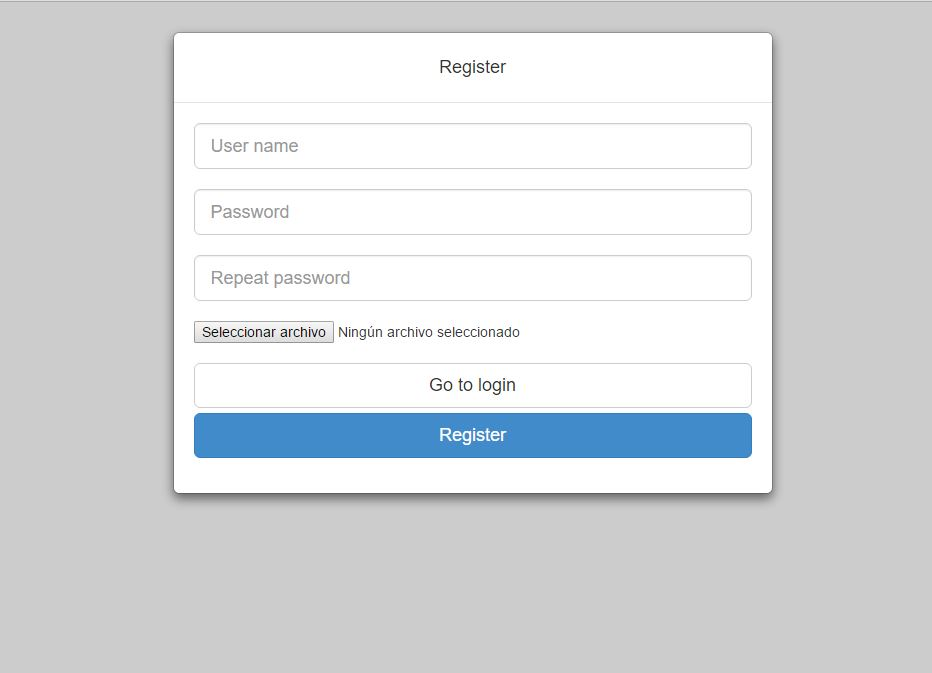
\includegraphics[scale=0.25]{imagenes/capitulo5/register.jpg}
	\caption{Crear un nuevo usuario}
	\label{img:AddUser}
\end{figure}

En este formulario tenemos que añadir el nombre del usuario, su contraseña y subir su imagen. Esta imagen aparecerá en el mapa del simulador. Una vez que hayamos creado el usuario tenemos que pulsar el botón "Go to login" para volver en la pantalla de login para introducir el nombre de nuestro usuario su contraseña.

\section{Actualizar el perfil de un usuario}

Para realizar cambios en el nombre del usuario, cambiar la imagen del perfil o cambiar la contraseña tenemos que ir en el menú Perfil:

\begin{figure}[H]
	\centering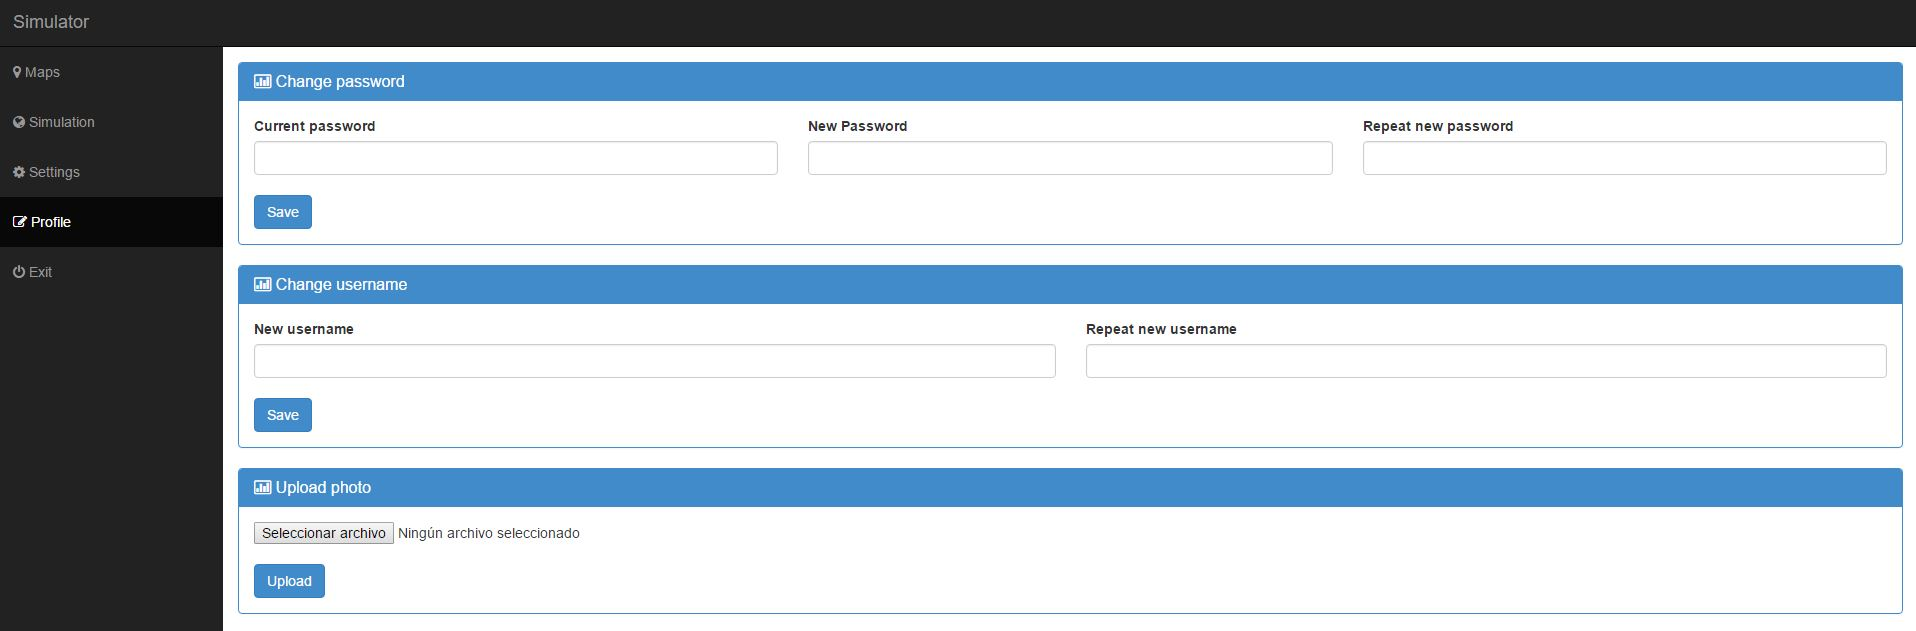
\includegraphics[scale=0.35]{imagenes/capitulo6/perfil-del-usuario.jpg}
	\caption{Actualizar el perfil de un usuario}
	\label{img:UpdateUser}
\end{figure}

Vemos que hay 3 formularios:

\begin{itemize}
	\item uno para cambiar el nombre del usuario
	\item otro para cambiar la contraseña del usuario
	\item otro para cambiar la imagen del perfil del usuarios
\end{itemize}

Al realizar cualquier cambio el el sistema nos informara si la acción ha salido bien o no.

\section{Búsqueda de mapas}\label{sec:BuscarMapas}

La opción Maps $\rightarrow$ map search nos permite buscar mapas a los cuales queremos conectarnos para realizar alguna simulación:

\begin{figure}[H]
	\centering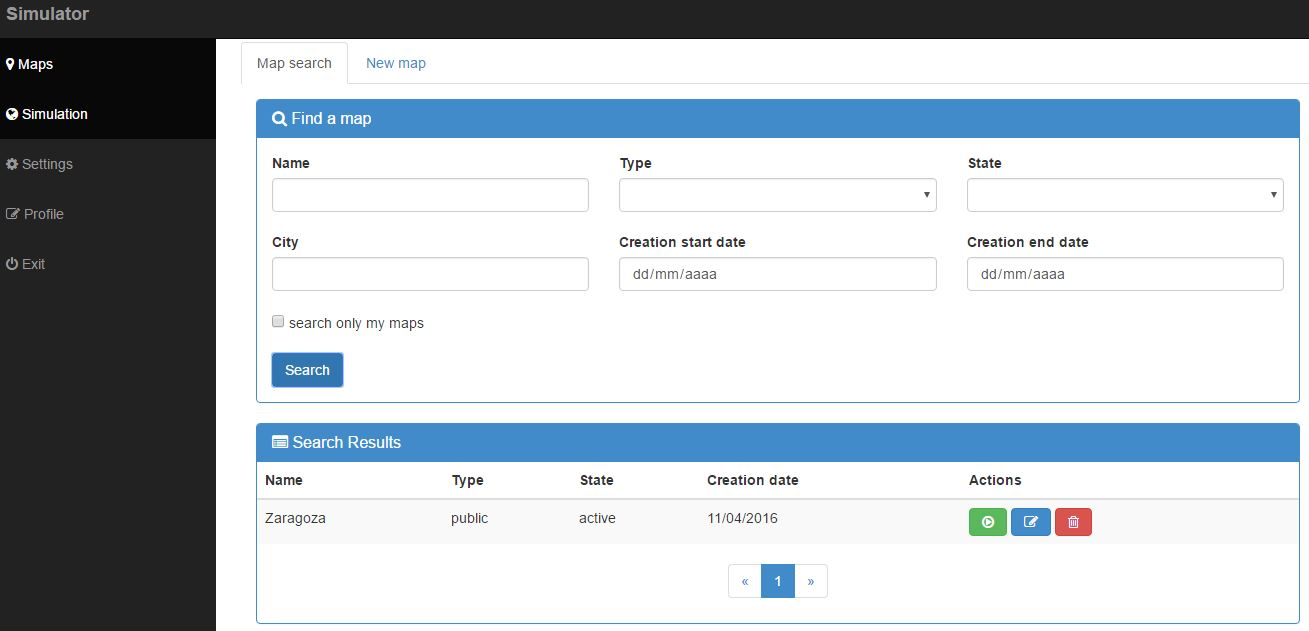
\includegraphics[scale=0.35]{imagenes/capitulo7/busqueda-de-mapas.jpg}
	\caption{Búsqueda de mapas}
	\label{img:BuscarMapas}
\end{figure}

En la imagen vemos que disponemos de distintos tipos de filtros para la búsqueda de mapas. Estos filtros son: por nombre, por tipo, por estado, por ciudad, por fechas de creación o solo buscar solo mis mapas. Si no introducimos ningún filtro devolverá todos los mapas que están creados en el sistema.

\section{Crear un nuevo mapa}\label{sec:crearMapa}

Para crear un nuevo mapa vamos en Maps $\rightarrow$ new map y vemos el siguiente formulario:

\begin{figure}[H]
	\centering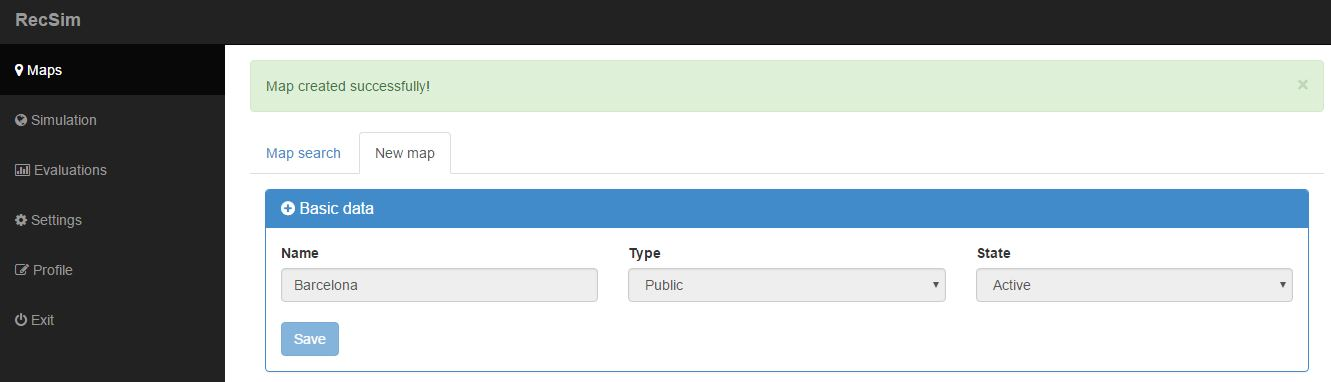
\includegraphics[scale=0.35]{imagenes/capitulo8/crear-un-nuevo-mapa.jpg}
	\caption{Crear un nuevo mapa}
	\label{img:AddMapa}
\end{figure}

Tenemos que rellenar los siguientes datos:

\begin{itemize}
	\item Name: es el nombre que queremos dar al mapa.
	\item Type: tipo que mapa. Podemos elegir entre publico (puede conectarse cualquier usuarios) y privado (solo puede conectarse el que la ha creado).
	\item State: estado del mapa. Podemos elegir entre activa (que el mapa está disponible para realizar simulaciones) y borrador (el mapa todavía no está disponible para realizar simulaciones)
\end{itemize}

Una vez que hayamos rellenado el formulario pulsamos en el botón Save y el sistema nos informara si el guardado ha salido con éxito o no. Si se ha guardado con éxito por debajo de este formulario aparece el formulario de creaciones de escenas y una lista de las escenas actuales. Lo normales es que la lista de escenas creadas aparezca vacía ya que todavía no hemos creado ninguna escena. Para ver los detalles de como crear una escena consultar el capítulo \ref{sec:crearEscena}.

\section{Crear una nueva escena}\label{sec:crearEscena}
Una vez que hayamos creado el mapa podemos empezar a crear las escenas. La creación de escenas se realiza en 4 pasos que vamos a ver a continuación.

\subsection{Paso 1: Elegir el nombre de la escena y el recomendador a utilizar}

En el primer paso tenemos que escoge un nombre para la escena que estamos configurando y elegir el tipo de recomendador que queremos usar el esta escena.

\begin{figure}[H]
	\centering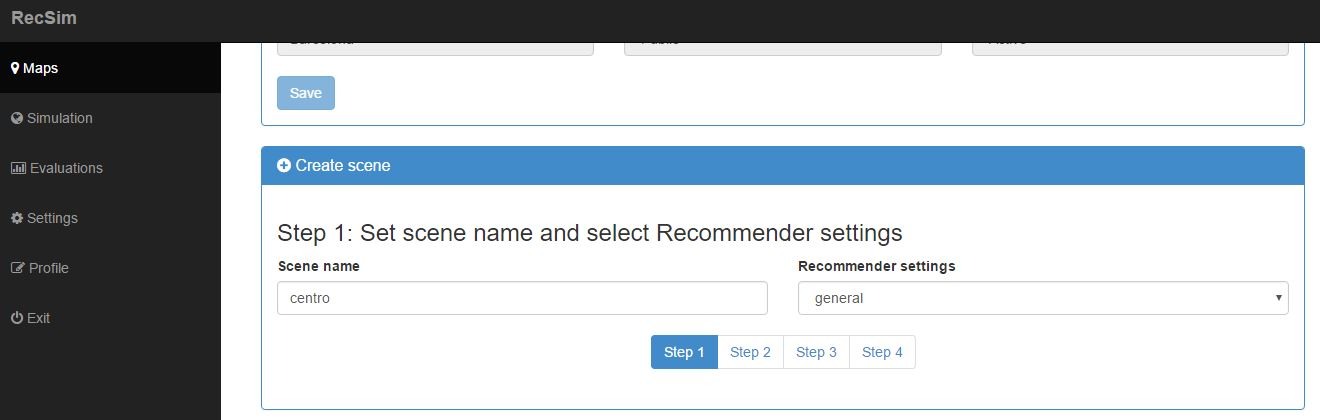
\includegraphics[scale=0.35]{imagenes/capitulo9/crear-escena-1.JPG}
	\caption{Paso 1: elegir nombre de la escena y el recomendador}
	\label{img:paso1}
\end{figure}

\subsection{Paso 2: Limites de la escena}

En este paso tenemos que buscar la ciudad donde se va a realizar la simulación y cuales son los limites de la escena.

\begin{figure}[H]
	\centering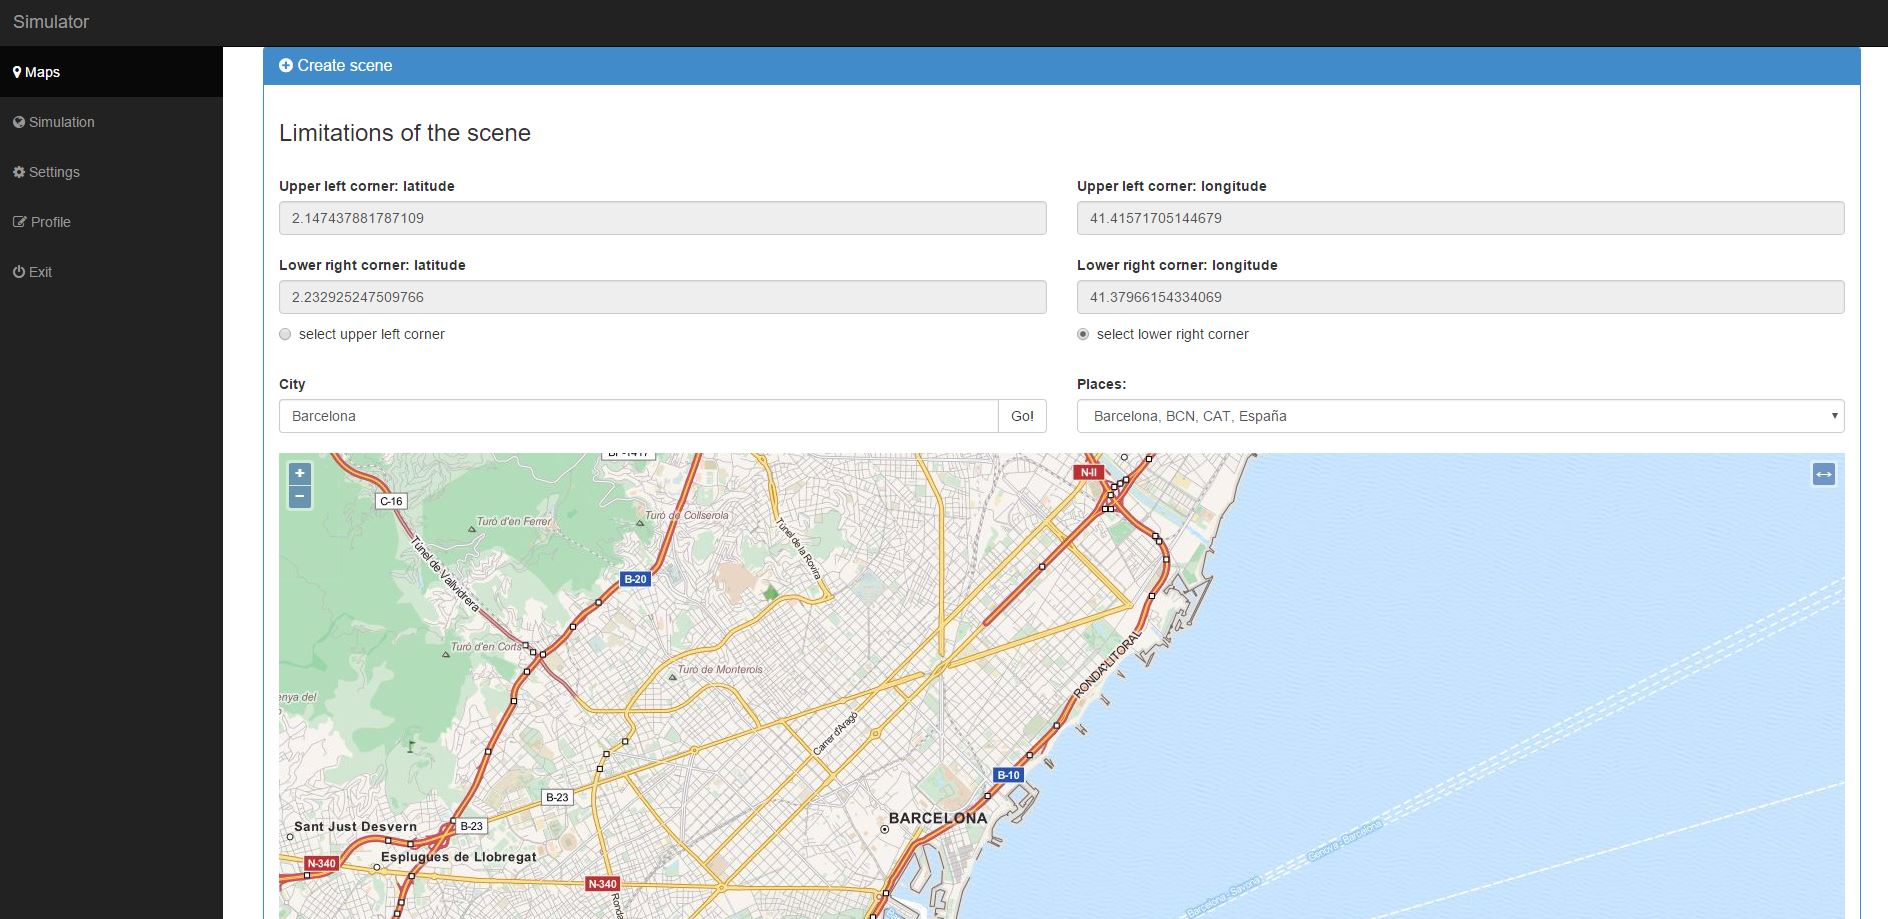
\includegraphics[scale=0.35]{imagenes/capitulo9/crear-escena-2.JPG}
	\caption{Paso 2: Limites de la escena}
	\label{img:paso2}
\end{figure}

Para buscar la cuidad donde se va a realizar la simulación tenemos poner cual es su nombre en la casilla City y pulsar el botón Go!. Vemos que al lado nos aparece un desplegable con una lista de resultados. Elegimos uno de ellos y vemos que el mapa que aparece al lado se actualiza.

Para definir los limites de la escena tenemos que establece cual es la esquina superior izquierda y la esquina inferior derecha. Para definir la esquina superior izquierda seleccionamos el select button select upper left corner y hacemos click en el mapa para definir donde estará dicha esquina. Veremos que las cajas de texto Upper left corner: latitude y Upper left corner: longitude aparecerán las coordenadas geográficas de dicha esquina (longitud y latitud).

Para definir la esquina inferior derecha seleccionamos la opción select lower right corner y hacemos click en el mapa para definir donde estará dicha esquina. Cuando hayamos seleccionado la esquina inferior derecha vemos que en las cajas de texto Lower right corner: latitude y Lower right corner: longitude aparecerán las coordenadas geográficas de dicha escena.


\subsection{Paso 3: Configurar los objetos estáticos}

Este paso consiste en definir cuales son los objetos estáticos y sus posiciones. Para definirlos disponemos de dos opciones: importarlos desde un fichero con formato JSON y deninirlos manualmente.

\subsubsection{Paso 3.1: importar los objetos estáticos}

Para importa los objetos estáticos seleccionamos la opciones load from file y nos aparecerá un formulario donde podemos elegir cual es el fichero que queremos importar. Antes de que se carguen los datos se nos previsualiza el contenido del fichero que queremos cargar:

\begin{figure}[H]
	\centering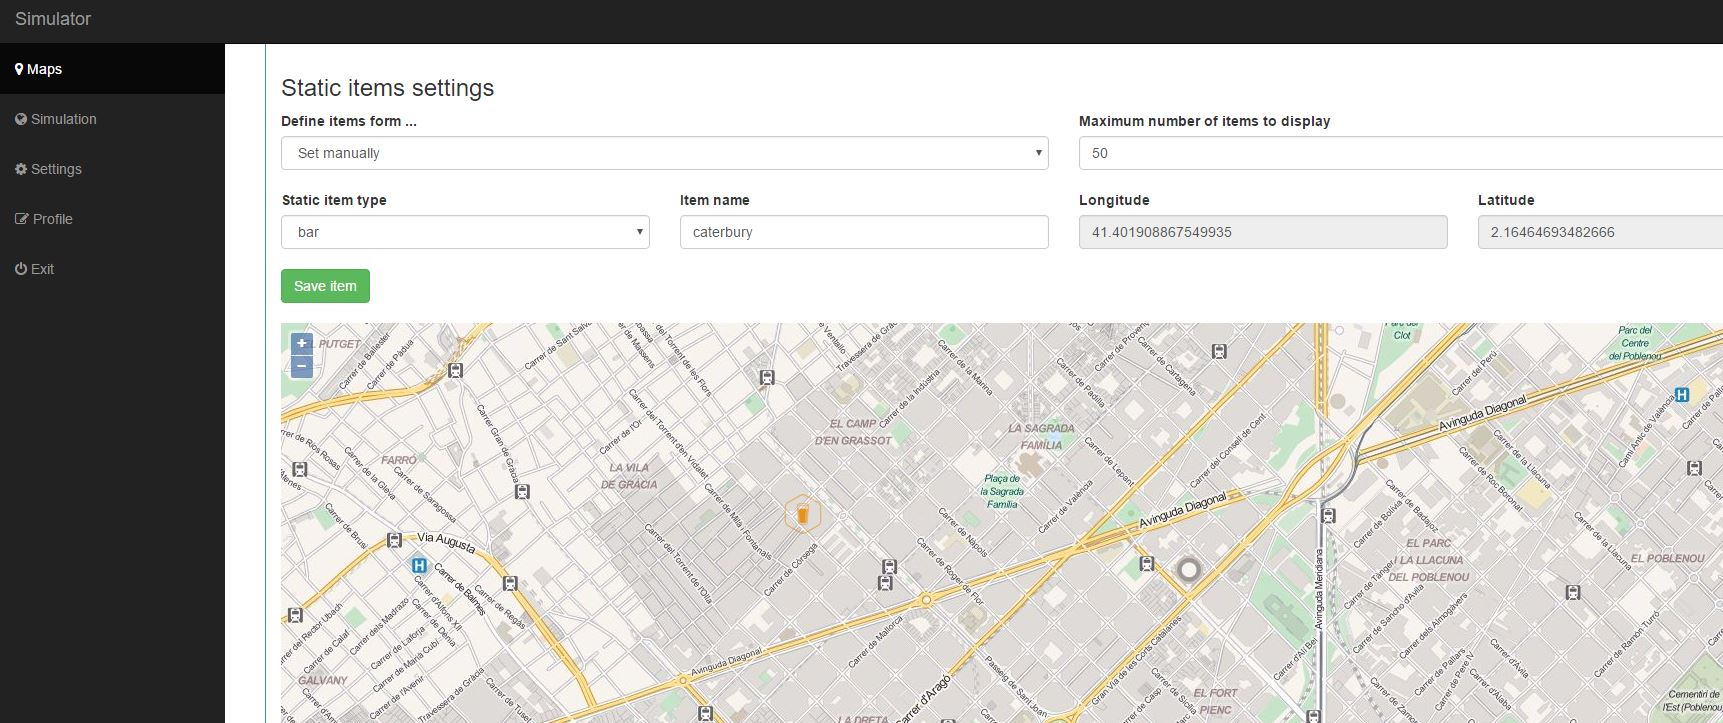
\includegraphics[scale=0.35]{imagenes/capitulo9/crear-escena-3-1.JPG}
	\caption{Paso 3.1: Previsualizar los objetos estáticos a importar}
	\label{img:paso3-1-1}
\end{figure}

En esta ventana tenemos que vincular los atributos del fichero a los atributos de nuestro sistema. Para cada atributo de nuestro sistema tenemos un select y en este select salen los atributos del fichero. Tenemos que seleccionar que atributo del fichero a que atributo de nuestro sistema queremos vincular. Por ultimo tenemos que elegir que tipo de objeto estático queremos asignar a los datos que estamos importando. Una vez importados los objetos nos aparecerá un table con todos los objetos importados.

\begin{figure}[H]
	\centering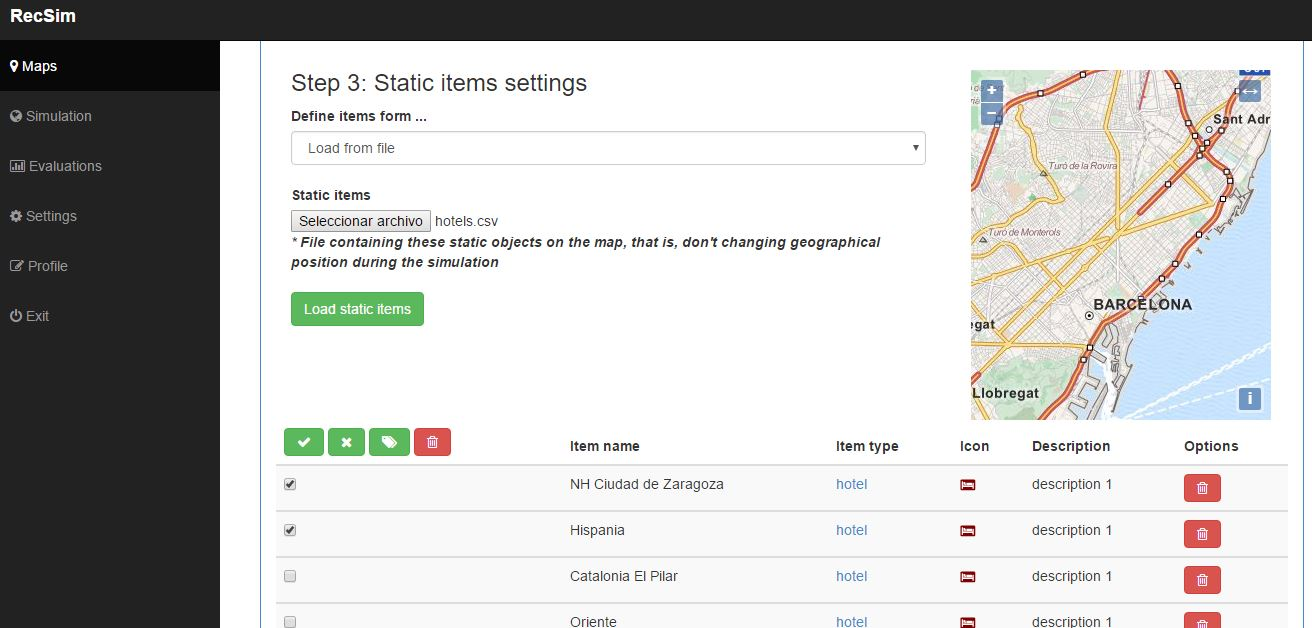
\includegraphics[scale=0.35]{imagenes/capitulo9/crear-escena-3.JPG}
	\caption{Paso 3.1: importar los objetos estáticos desde un fichero}
	\label{img:paso3-1}
\end{figure}

Una vez importados los objetos vemos que disponemos una serie de opciones que nos permiten gestionar los objetos importados. Podemos seleccionar un subconjunto y todos los objetos y cambiarles el tipo o borrarles. Esto se hace con las opciones que tenemos en la cabecera de la tabla.

\subsubsection{Paso 3.2: definir los objetos estáticos manualmente}

Para definirlos de forma manual tenemos que seleccionar la opción set manually y nos aparecer un formulario con el tipo de item que queremos definir, el nombre que queremos asignarle. Para definir cuales son sus coordenadas geográficas tenemos que seleccionar la posiciones directamente sobre el mapa. A continuación pulsamos sobre el botón Save Item y nos aparecerá la misma tabla que el en paso 3.1:

\begin{figure}[H]
	\centering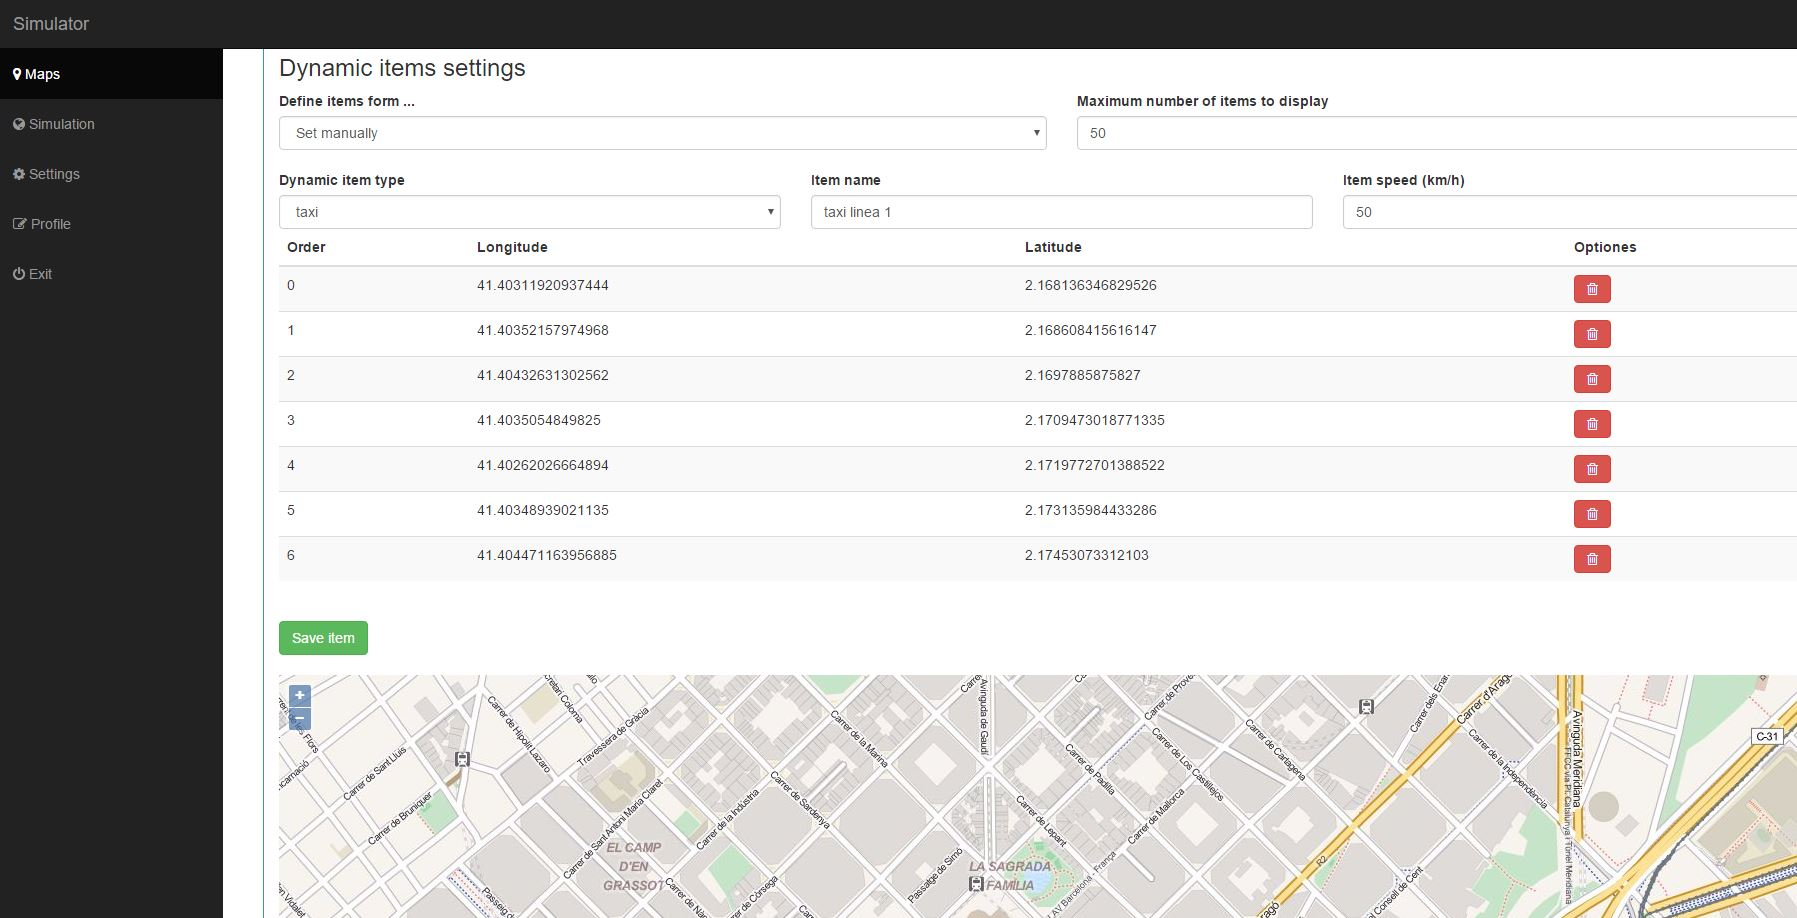
\includegraphics[scale=0.35]{imagenes/capitulo9/crear-escena-4.JPG}
	\caption{Paso 3.2:  definir los objetos estáticos manualmente}
	\label{img:paso3-2}
\end{figure}

\subsection{Paso 4: Configurar los objetos dinámicos}

El últimos paso consiste en definir los objetos dinámicos y sus rutas. Disponemos de 3 posibles maneras para definirlos: importándolos desde un fichero con formato JSON, definirlos manualmente, generarlos aleatoriamente.

\subsubsection{Paso 4.1: importar los objetos dinámicos}

Para importarlos objetos dinámicos desde un fichero tenemos que seleccionar la opción load from file y nos aparecerá un formulario que nos permite seleccionar el fichero a importar. Antes de cargar los objetos dinámicos podemos previsualizar los datos y vincular los atributos del fichero a los atributos del sistema. Esto se realiza mediante los selects que observamos en la siguiente pantalla:

\begin{figure}[H]
	\centering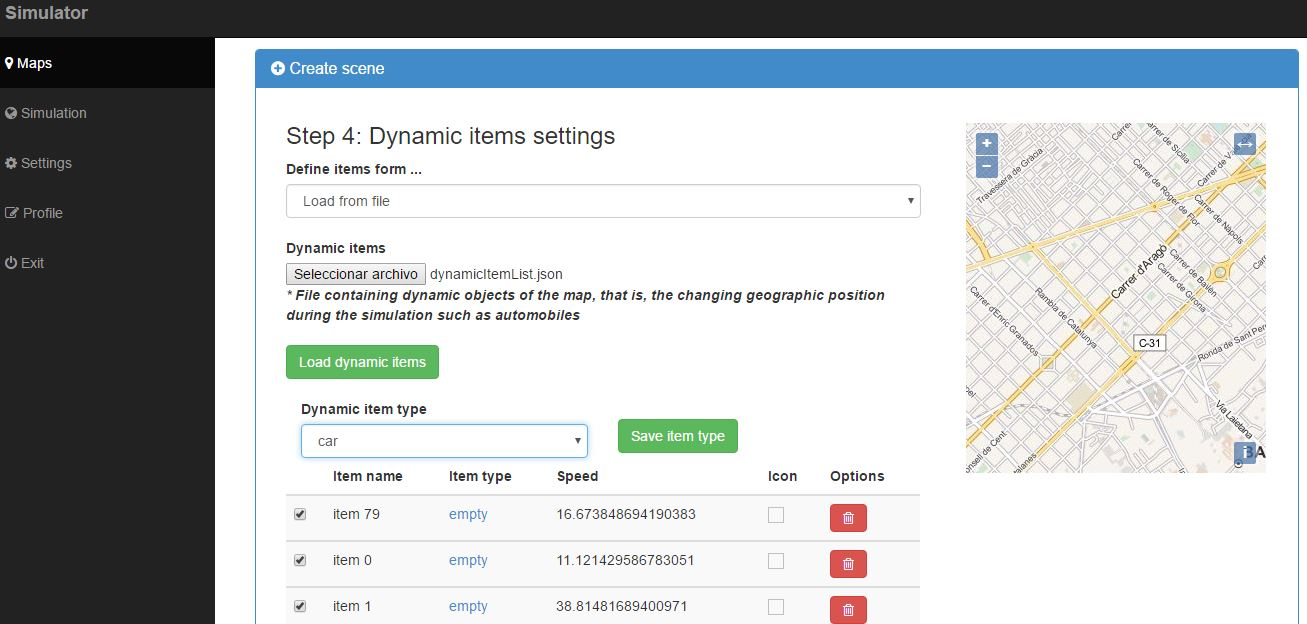
\includegraphics[scale=0.35]{imagenes/capitulo9/crear-escena-8.JPG}
	\caption{Paso 4.1: importar los objetos dinámicos}
	\label{img:paso4-1}
\end{figure}

Una vez que hayamos importado los ficheros vemos una tabla parecida que tabla del paso 3.1. La diferencia es que aquí disponemos de más opciones. Entre estas opciones son las de generar las rutas a un subconjunto a todos los datos, cambiar el tipo de objeto dinámico y borrarlos objetos seleccionados.

\subsubsection{Paso 4.2: definir los objetos dinámicos manualmente}

Para definir los objetos dinámicos manualmente seleccionamos la opción set manually nos aparecer un formulario en el cual tenemos que elegir el tipo de objeto dinámico, el nombre que queremos asignarle y su velocidad. Para definir la trayectoria de este tenemos que seleccionar los nodos del grafo de movimiento directamente en el mapa y nos aparecerá una tabla que contiene dichos nodos:

\begin{figure}[H]
	\centering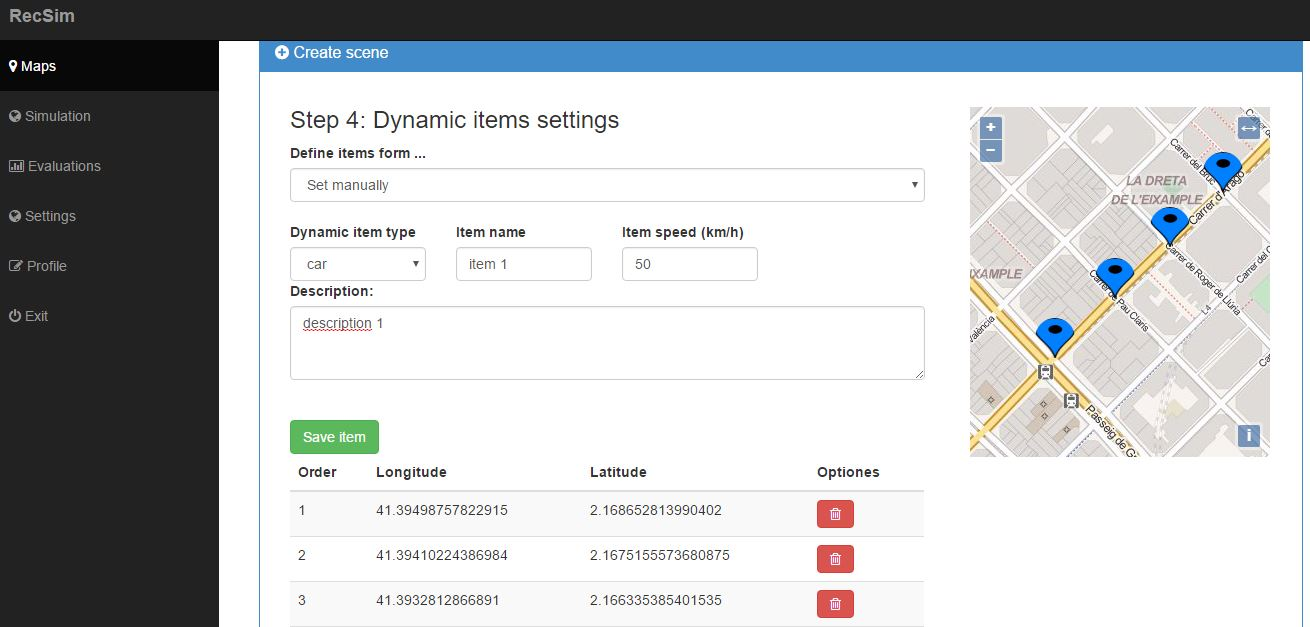
\includegraphics[scale=0.35]{imagenes/capitulo9/crear-escena-6.JPG}
	\caption{Paso 4.2: definir los objetos dinámicos manualmente}
	\label{img:paso4-2-1}
\end{figure}

Una vez que hayamos definido el trayecto pulsamos sobre el botón Save item y nos saldrá la lista con todos los objetos dinámicos en la escena:

\begin{figure}[H]
	\centering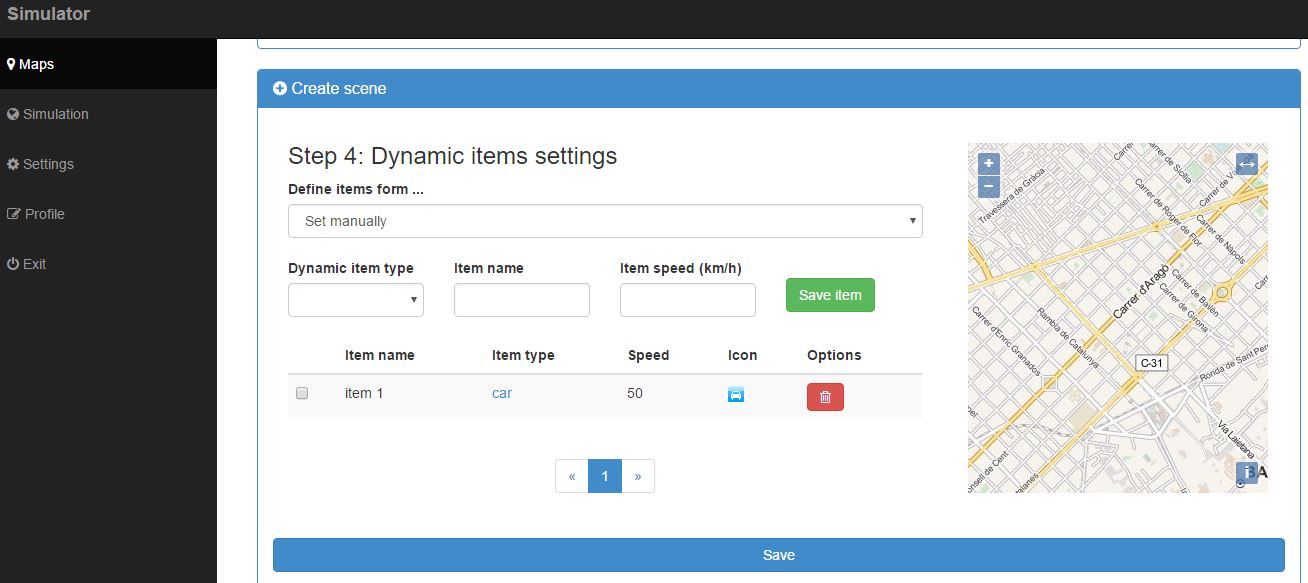
\includegraphics[scale=0.35]{imagenes/capitulo9/crear-escena-7.JPG}
	\caption{Paso 4.2: definir los objetos dinámicos manualmente}
	\label{img:paso4-2-2}
\end{figure}

\subsubsection{Paso 4.3: generar los objetos dinámicos aleatoriamente}

Para generar los trayectos de forma aleatoria tenemos que seleccionar la opción Random trajectory y aparecerá un formulario donde tenemos que indicar el tipo de objeto dinámico que queremos generar, la cantidad de objetos que queremos generar y el tipo de vía en la que queremos que aparezcan. A continuación pulsamos sobre el botón Generate random way y tenemos que esperar que se generen las rutas. Este proceso puede ser bastante costoso y tenemos que ser pacientes. Esto es debido porque se baja el grafo de la escena y este pesa algunos cuantos megas.

\begin{figure}[H]
	\centering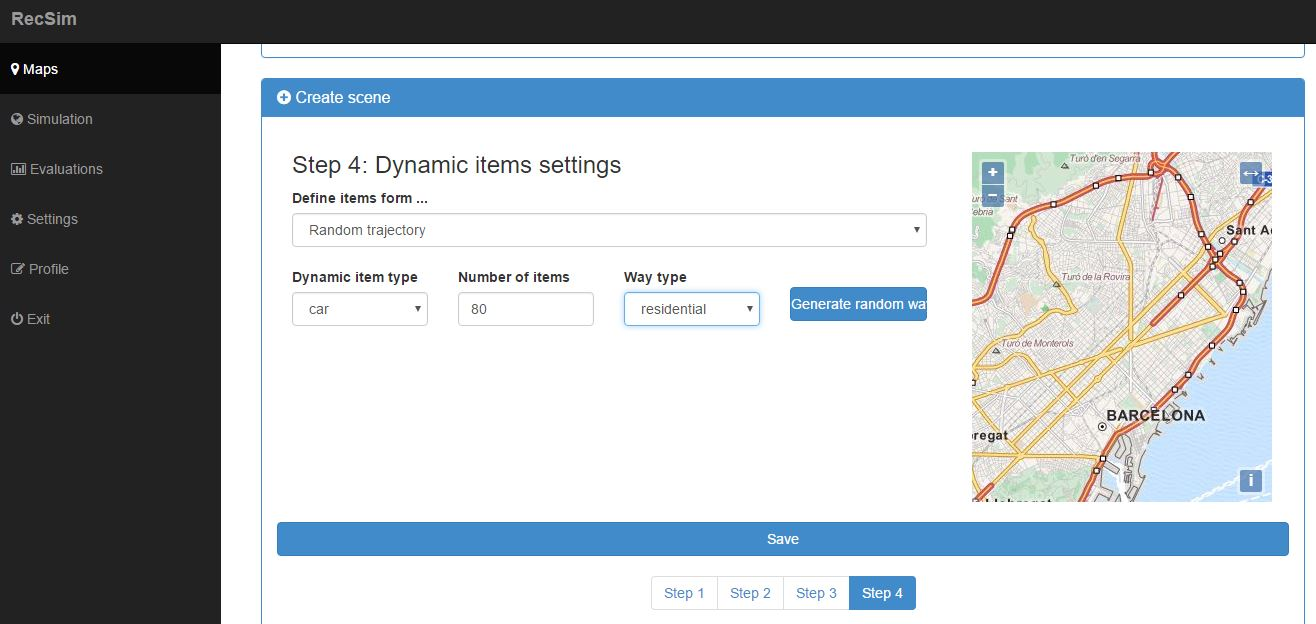
\includegraphics[scale=0.35]{imagenes/capitulo9/crear-escena-5.JPG}
	\caption{Paso 4.3: generar los objetos dinámicos aleatoriamente}
	\label{img:paso4-3}
\end{figure}

\section{Edición de mapas y escenas}\label{sec:editarMapasEscenas}

Para modificar un mapa o escena primero tenemos que realizar una busque de mapas en Maps $\rightarrow$ maps search y en la lista de resultados pulsamos sobre el icono de editar imagen. Solo podemos editar un mapa si la hayamos creado nosotros. De lo contrario el icono de editar imagen no aparecerá. Una vez que hayamos pulsado el icono de editar imagen entonces veremos la siguiente pantalla:

\begin{figure}[H]
	\centering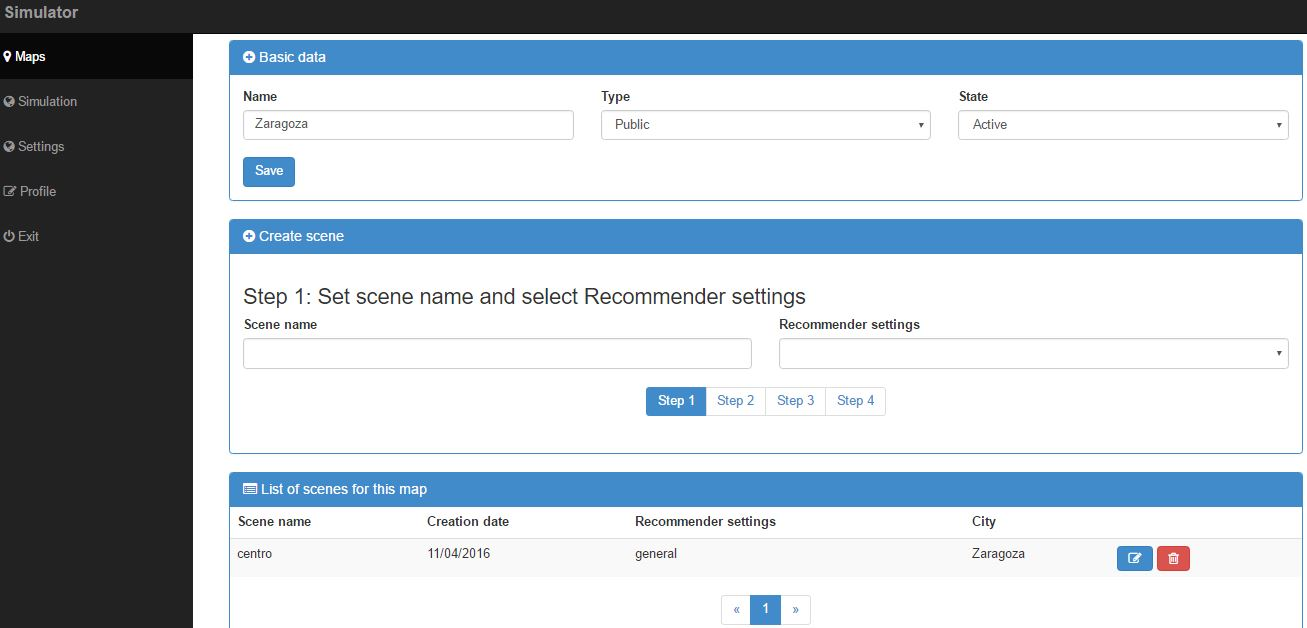
\includegraphics[scale=0.35]{imagenes/capitulo10/capitulo10.jpg}
	\caption{Edición de mapas y escenas}
	\label{img:UpdateMapScene}
\end{figure}

En esta pantalla disponemos de distintos tipos de opciones entre los cuales modificar datos del mapa, crear o modificar escenas.

\section{Simulación}

Para ejecutar una simulación lo primero que tenemos que hacer es realizar la búsqueda de un mapa explicado en el capítulo \ref{sec:BuscarMapas}. Una vez que hayamos realizado la búsqueda pulsamos el botón "Play" y a continuación se nos muestra una pantalla en la cual tenemos que elegir la escena a la cual queremos conectarnos.

\begin{figure}[H]
	\centering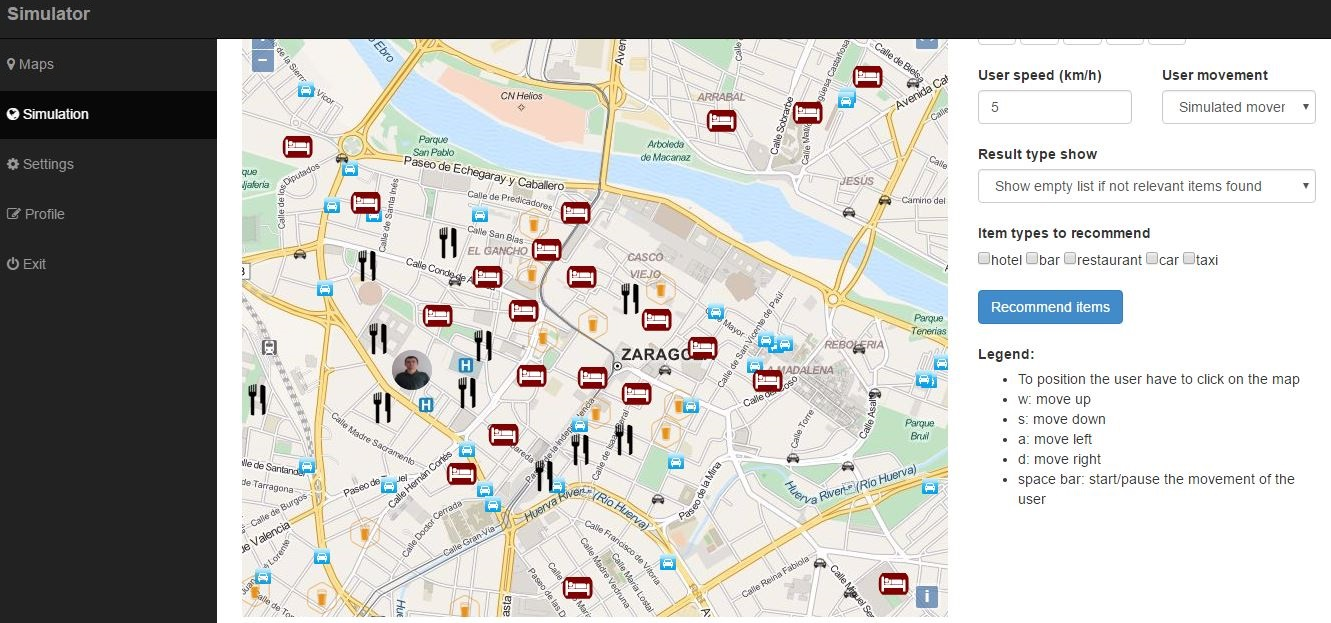
\includegraphics[scale=0.35]{imagenes/capitulo11/capitulo11.jpg}
	\caption{Simulación}
	\label{img:Simulation}
\end{figure}

Para iniciar la simulación y que todos los items empiecen a moverse tenemos que pulsar el botón play. Hay que tener en cuenta que existe la posibilidad que de ya haya usuario que estén ejecutando una simulación sobre este escenario. Por esto cuando nos conectemos a la escena veremos que los objetos ya se estén moviendo. En cualquier momento podemos pausar la simulación. Entonces la simulación se pausa en todos los usuarios que están conectados en la escena. En cualquier momento cualquier usuario puede reanudar la simulación. Para salir de la simulación lo único que tenemos que hacer es salir de la pantalla de simulación.

\subsection{Controles del usuario}

Una vez cargada la escena podemos elegir entre usar la posición GPS del dispositivo con el cual nos estamos conectado y simular los movimientos del usuario.

\subsubsection{Coordenadas GPS}

Para usar el posicionamiento por GPS tenemos que elegir GPS positioning en el select con nombre User movement y nuestro icono aparecerá en el mapa. A medida que nos vamos moviendo vemos que nuestra posición se va actualizando.

\subsubsection{Movimiento simulado}

Para usar el movimiento simulado tenemos que elegir Simulated movement en el select con nombre User movement y a continuación tenemos que elegir donde queremos situarnos en el mapa haciendo click en el mapa. A continuación podemos empezar a movernos por el mapa con los siguientes controles:s

\begin{itemize}
	\item tecla w: movimiento hacia arriba
	\item tecla s: movimiento hacia abajo
	\item tecla a: movimiento hacia la izquierda
	\item tecla d: movimiento hacia la derecha
	\item espacio: pausar el movimiento del usuario
\end{itemize}

\subsection{Recomendaciones}

Para obtener recomendaciones tenemos que seguir los siguientes pasos:

\begin{itemize}
	\item paso 1: seleccionamos los tipos de items sobre los cuales queremos obtener resultados (items types to recommend)
	\item paso 2: en Result type show elegimos como queremos que se nos muestren los resultados. Por defecto si el recomendador no tiene items que recomendar mostrará una lista vacía.
	\item paso 3: pulsamos el botón Recommend items para obtener resultados
\end{itemize}

\subsection{Votaciones}

Para realizar las votaciones disponemos de los siguientes opciones:

\begin{itemize}
	\item opción 1: pulsamos sobre el item concreto en el mapa y se nos abrirá una select donde podemos votar
	\item opción 2: una vez que hayamos obtenido una lista con items recomendados disponemos de un select donde podemos realizar la votación
\end{itemize}

\newpage

\section{Evaluación de un recomendador}

Para realizar la evaluación de un recomendador vamos en el menú Evaluations:

\begin{figure}[H]
	\centering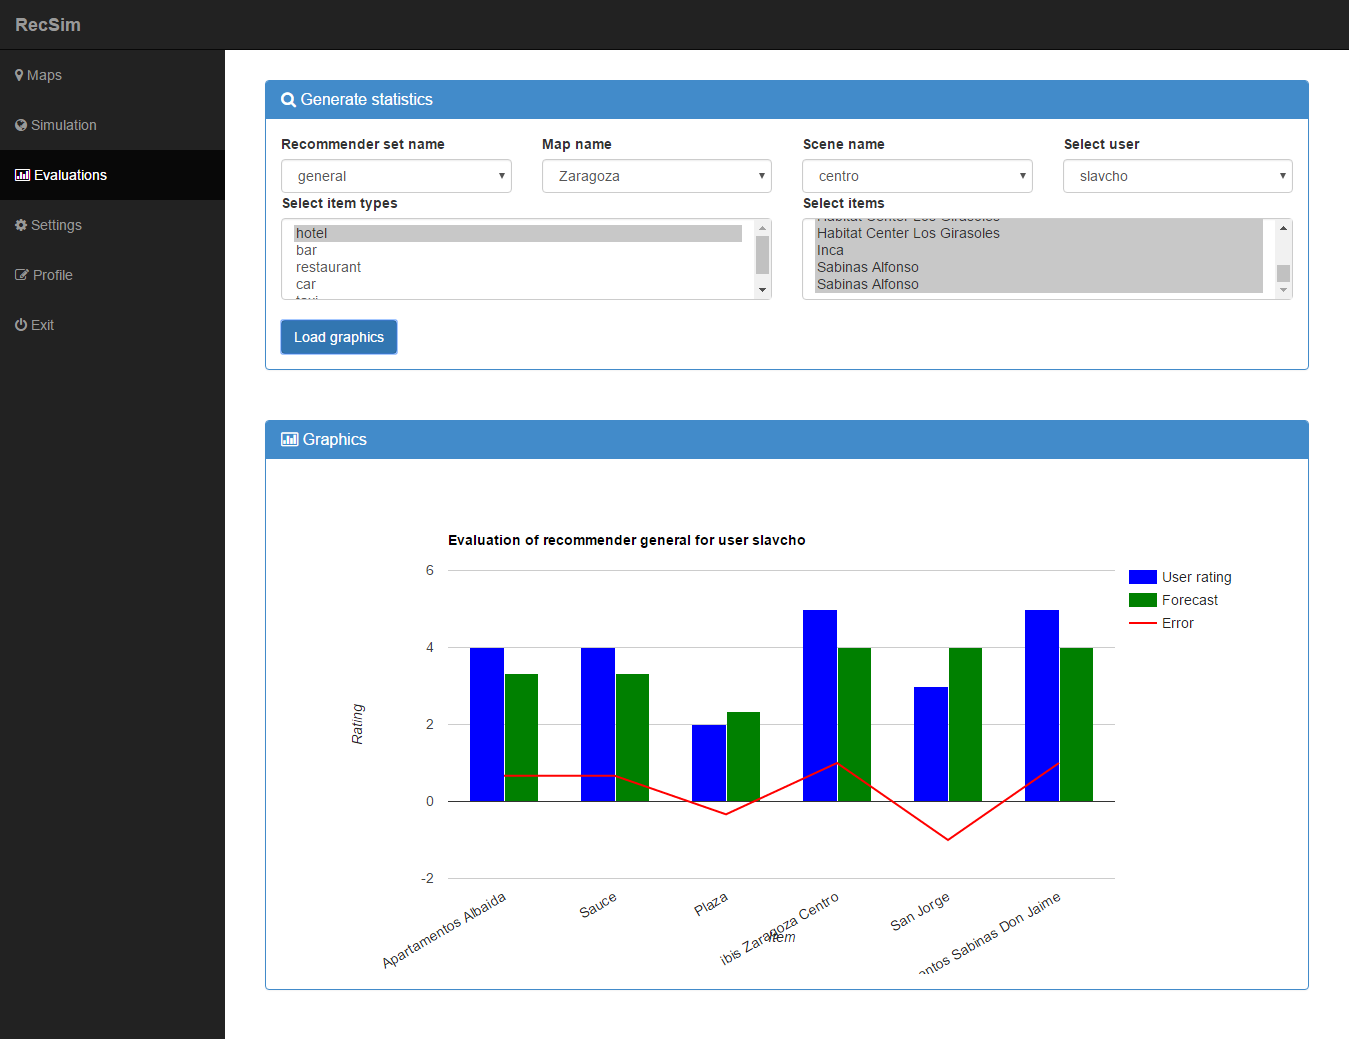
\includegraphics[scale=0.35]{imagenes/capitulo12/evaluacion.png}
	\caption{Evaluación de un recomendador}
	\label{img:evaluacion}
\end{figure}

Lo primero que tenemos que hacer es seleccionar el tipo de recomendador que queremos evaluar. Una vez que hayamos seleccionado el tipo de recomendador nos aparecen los mapas y escenas donde se utiliza este. A continuación tenemos que seleccionar el usuario que queremos evaluar y escoger una lista de items. Al final pulsamos el botón Load Graphics y se muestra un gráfico con el item, la valoración que ha dato el usuario, el valor estimado en este momento y el error. Si no disponemos de datos de algún item este no saldrá en el gráfico. Si no disponemos de ningún dato se nos indicara con un mensaje.
